\documentclass[]{article}


\usepackage{graphicx,forloop,caption,subcaption,float,hyperref,arrayjob,listings,color,booktabs,mathtools}
\usepackage{pdfpages}
\usepackage{amsmath}
\usepackage{multirow}
%vhdl code
\definecolor{dkgreen}{rgb}{0,0.6,0}
\definecolor{gray}{rgb}{0.5,0.5,0.5}
\definecolor{mauve}{rgb}{0.58,0,0.82}

\DeclareMathOperator*{\argmin}{\arg\!\min}


\lstset{frame=tb,
  language=VHDL,
  aboveskip=3mm,
  belowskip=3mm,
  showstringspaces=false,
  columns=flexible,
  basicstyle={\small\ttfamily},
  numbers=none,
  numberstyle=\tiny\color{gray},
  keywordstyle=\color{blue},
  commentstyle=\color{dkgreen},
  stringstyle=\color{mauve},
  breaklines=true,
  breakatwhitespace=true
  tabsize=3
}

%matlab code
\lstset{frame=tb,
  language=Matlab,
  aboveskip=3mm,
  belowskip=3mm,
  showstringspaces=false,
  columns=flexible,
  basicstyle={\small\ttfamily},
  numbers=none,
  numberstyle=\tiny\color{gray},
  keywordstyle=\color{blue},
  commentstyle=\color{dkgreen},
  stringstyle=\color{mauve},
  breaklines=true,
  breakatwhitespace=true
  tabsize=3
}


% Title Page
\title{UCLA\\EE230B\\Digital Communication Design Project\\Step 1 Report}
\author{Alican Salor 404271991 \\  \href{mailto:alicansalor@ucla.edu}{alicansalor@ucla.edu} \\ \\
Darren Reis 804359840 \\
\href{mailto:darrer.r.reis@gmail.com}{darren.r.reis@gmail.com} }


\begin{document}
\maketitle

\newpage
\tableofcontents

\newpage


\section{System Setup}
\label{sec:setup}
The system is as shown in Figure BLAH.  To simulate the system, code was written for each block in the diagram.  A random bit generator was used to output a stream of data (Appendix~\ref{app:random_bit_generator}).  The data stream then was passed into a bit-to-symbol mapper, transformed differently based on the modulation scheme (Appendix~\ref{app:bittosym}).  Various schemes were used, including Binary Phase Shift Keying [BPSK], Quadrature Phase Shift Keying [QPSK], and Quadrature Amplitude Modulation [QAM], as shown in Appendices~\ref{app:bpsk_mod}~$-$~\ref{app:qam_64_mod}. To approximate a real system, the system got passed through a square root raised cosine pulse (Appendix~\ref{app:sqrt_raised_cosine}).  This filter was then oversampled by four in order to DO BLAH (Appendix~\ref{app:impulse_train}).  To simulate world noises, it was broadcast over a channel of additive white gaussian noises (Appendix~\ref{app:awgn_channel}).  For different SNR levels, the AWGN channel had different gain and variance.  This channel modeled the transmission of the signal from transmitter to receiver.  The receiver then used a matched filter version of the raised cosine pusle-shape.  After sampling the symbol stream back at the original symbol rate, the message was ready for recovery (Appendix~\ref{app:sampler}).  Finally, the data waveform was sent through a decision block, demodulating according to the appropriate scheme (Appendices~\ref{app:bpsk_demod}~$-$~\ref{app:qam_64_demod}).  

An analysis of performance of the system was determined by comparing a theoretical error rate to experimental bit error rate for various schemes.  The theoretical derivation is shown in Section~\ref{sec:deriv}.  The experimental error rate was found by counting the instances of wrongly decoded bits.  


\section{Mathematical Derivations of Probability of Error}
\label{sec:deriv}
As equiprobable bits are generated thou

\subsection{BPSK}
\label{sec:bpsk}

As equiprobable bits are generated and passed through an AWGN channel in this project we have used ML decision rule which states: \\

$\hat{m} = \argmin_{1\leq m \leq M}{||\underline{r} - \underline{s}_m||}$ 
\\

Thus in the following subsections the probability of error for each constellation used in the project is derived using the minimum distance rule.


\subsection{BPSK}
The exact probability of bit error is as follows (no interseting decision regions):

$ P_e = Q(\frac{d_{min}/2}{\sqrt{N_o/2}}) $
$       = Q(\sqrt{\frac{2E_b}{N_o}}) $

\subsection{QPSK}
\label{sec:qpsk}

The exact probability of bit error is as follows (found by subtracting the interseting decision regions from the nearest neighbour approx.):

$ P_e = Q(\frac{d_{min}/2}{\sqrt{N_o/2}}) $
$       = Q(\sqrt{\frac{2E_s}{N_o}}) $ 

\subsection{16-QAM}
\label{sec:qam16}




The exact probability of bit error is as follows (found by subtracting the interseting decision regions from the nearest neighbour approx.):

$ P_e = Q(\frac{d_{min}/2}{\sqrt{N_o/2}}) \\$
$       = 3Q(\sqrt{\frac{4}{5}\frac{E_b}{N_o}})-(9/4)Q(\sqrt{\frac{4}{5}\frac{E_b}{N_o}}))^2$ 

\subsection{64-QAM}
\label{sec:qam64}
The exact probability of bit error is as follows (found by subtracting the interseting decision regions from the nearest neighbour approx.):

$ P_e = Q(\frac{d_{min}/2}{\sqrt{N_o/2}}) $
$       = Q(\sqrt{\frac{2E_s}{N_o}}) $ 


\appendix
\newpage
% the \\ insures the section title is centered below the phrase: Appendix B
\section{Project Assignment}
\label{app:assign}
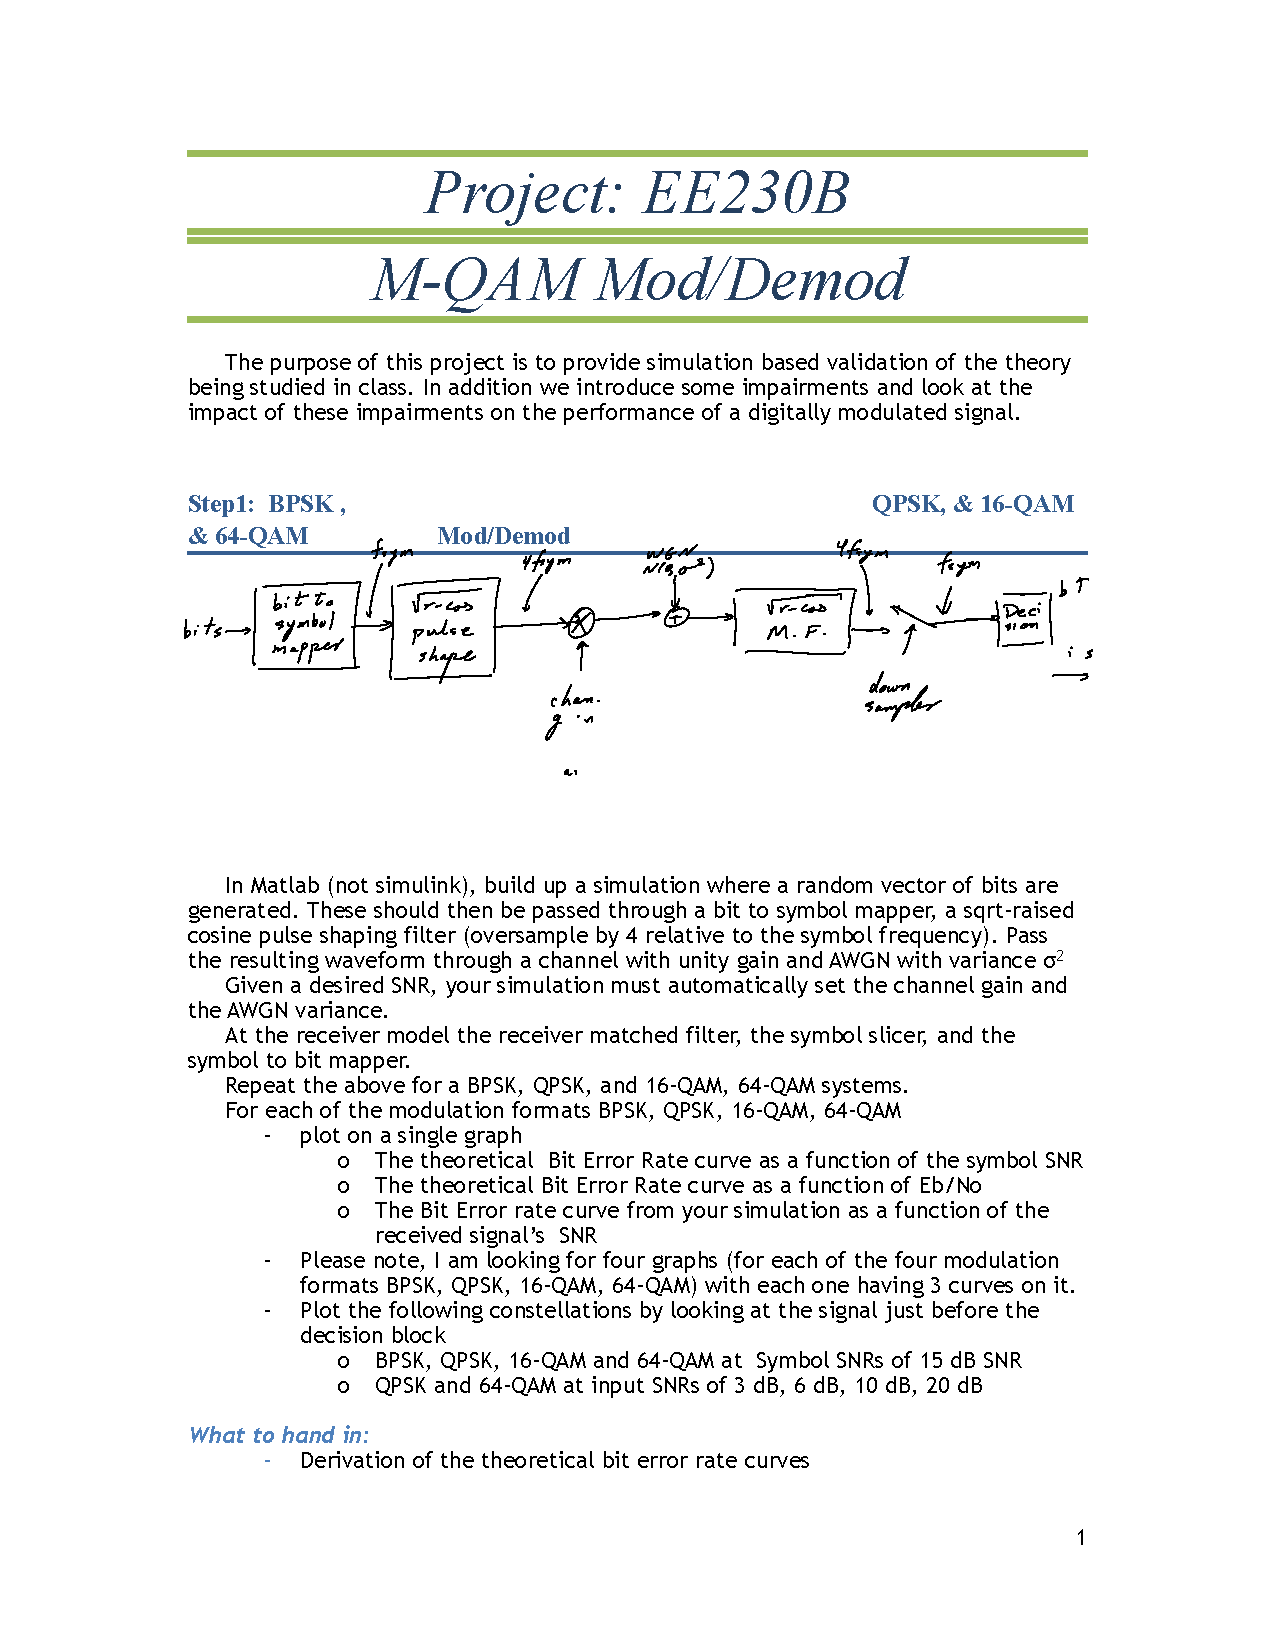
\includepdf[pages={1-5}]{project_overview.pdf}
\cleardoublepage
\newpage


\section{Random Bit Sequence Generator}
\label{app:random_bit_generator}
\lstinputlisting{random_bit_generator.m}
\cleardoublepage
\newpage

\section{Bit to Symbol Mappers}
\label{app:bittosym}
\subsection{BPSK Modulation }
\label{app:bpsk_mod}
% To convert program (e.g. C++ Fortran, Matlab, LaTeX) listings to a
% form easily includable in a LaTeX document
%
% type lgrind -s to see options
% lgrind -llatex -i sample-paper.tex > sampleinputtex
% creates a file sampleinput.tex which can then be included into this
% document simply by uncommenting the next line
%\lgrindfile{testinput.tex}

\lstinputlisting{bpsk_mod.m}
\cleardoublepage  % force onto odd page
\newpage

\subsection{QPSK Modulation}
\label{app:qpsk_mod}
\lstinputlisting{qpsk_mod.m}
\cleardoublepage  % force onto odd page
\newpage

\subsection{16-QAM Modulation}
\label{app:qam_16_mod}

\lstinputlisting{QAM_16_mod.m}
\cleardoublepage  % force onto odd page
\newpage

\subsection{64-QAM Modulation }
\label{app:qam_64_mod}
\lstinputlisting{QAM_64_mod.m}
\cleardoublepage  % force onto odd page
\newpage

\section{Square Root Raised Cosine Filter}
\label{app:sqrt_raised_cosine}
\lstinputlisting{sqrt_raised_cosine.m}
\cleardoublepage
\newpage

\section{Up Sampler}
\label{app:impulse_train}
\lstinputlisting{impulse_train.m}
\cleardoublepage
\newpage

\section{Additive Gaussian White Noise Channel}
\label{app:awgn_channel}
\lstinputlisting{awgn_channel.m}
\cleardoublepage
\newpage

\section{Additive Gaussian White Noise Channel}
\label{app:awgn_channel}
\lstinputlisting{awgn_channel.m}
\cleardoublepage
\newpage

\section{Sampler}
\label{app:sampler}
\lstinputlisting{sampler.m}
\cleardoublepage
\newpage

\section{Decision Blocks}
\label{app:dblocks}
\subsection{BPSK Demodulation}
\label{app:bpsk_demod}
\lstinputlisting{bpsk_demod.m}
\cleardoublepage
\newpage

\subsection{QPSK Demodulation}
\label{app:qpsk_demod}
\lstinputlisting{qpsk_demod.m}
\cleardoublepage
\newpage

\subsection{16-QAM Demodulation}
\label{app:qam_16_demod}
\lstinputlisting{QAM_16_demod.m}
\cleardoublepage
\newpage

\subsection{64-QAM Demodulation}
\label{app:qam_64_demod}
\lstinputlisting{QAM_64_demod.m}
\cleardoublepage
\newpage

\end{document}
